\section{Technical Overview}

\subsection{Topology and Upstream Connectivity}

Building an Internet Service Provider means connecting your network to
as many others as possible. To do this means being present at places
where other networks are present. In Scotland this means the Scolocate
and IOMart datacentres in Edinburgh and Glasgow. These are not as big as
the corresponding places in Manchester and London, but are growing,
and being present there means being able to make whatever arrangements
are necessary to obtain \textit{transit} to the rest of the Internet
from larger, tier 1 and tier 2 providers that are also there.

So this is why we separate out two concerns: getting to the exchange
points and data centres, and getting from those data centres to the
Internet. By separating out these concerns we are not locked into a
single choice made at the beginning about who we will get ``Internet
backhaul'' from. As the landscape changes, and providers come and go,
these choices can be changed, at will, without having to change the
internal details of our networks. Our network is autonomous and can
treat with other neighbour networks as an entity in its own
right. This is future-proofing and is not something that is possible
by just buying Internet access.

\begin{figure}
  \begin{center}
    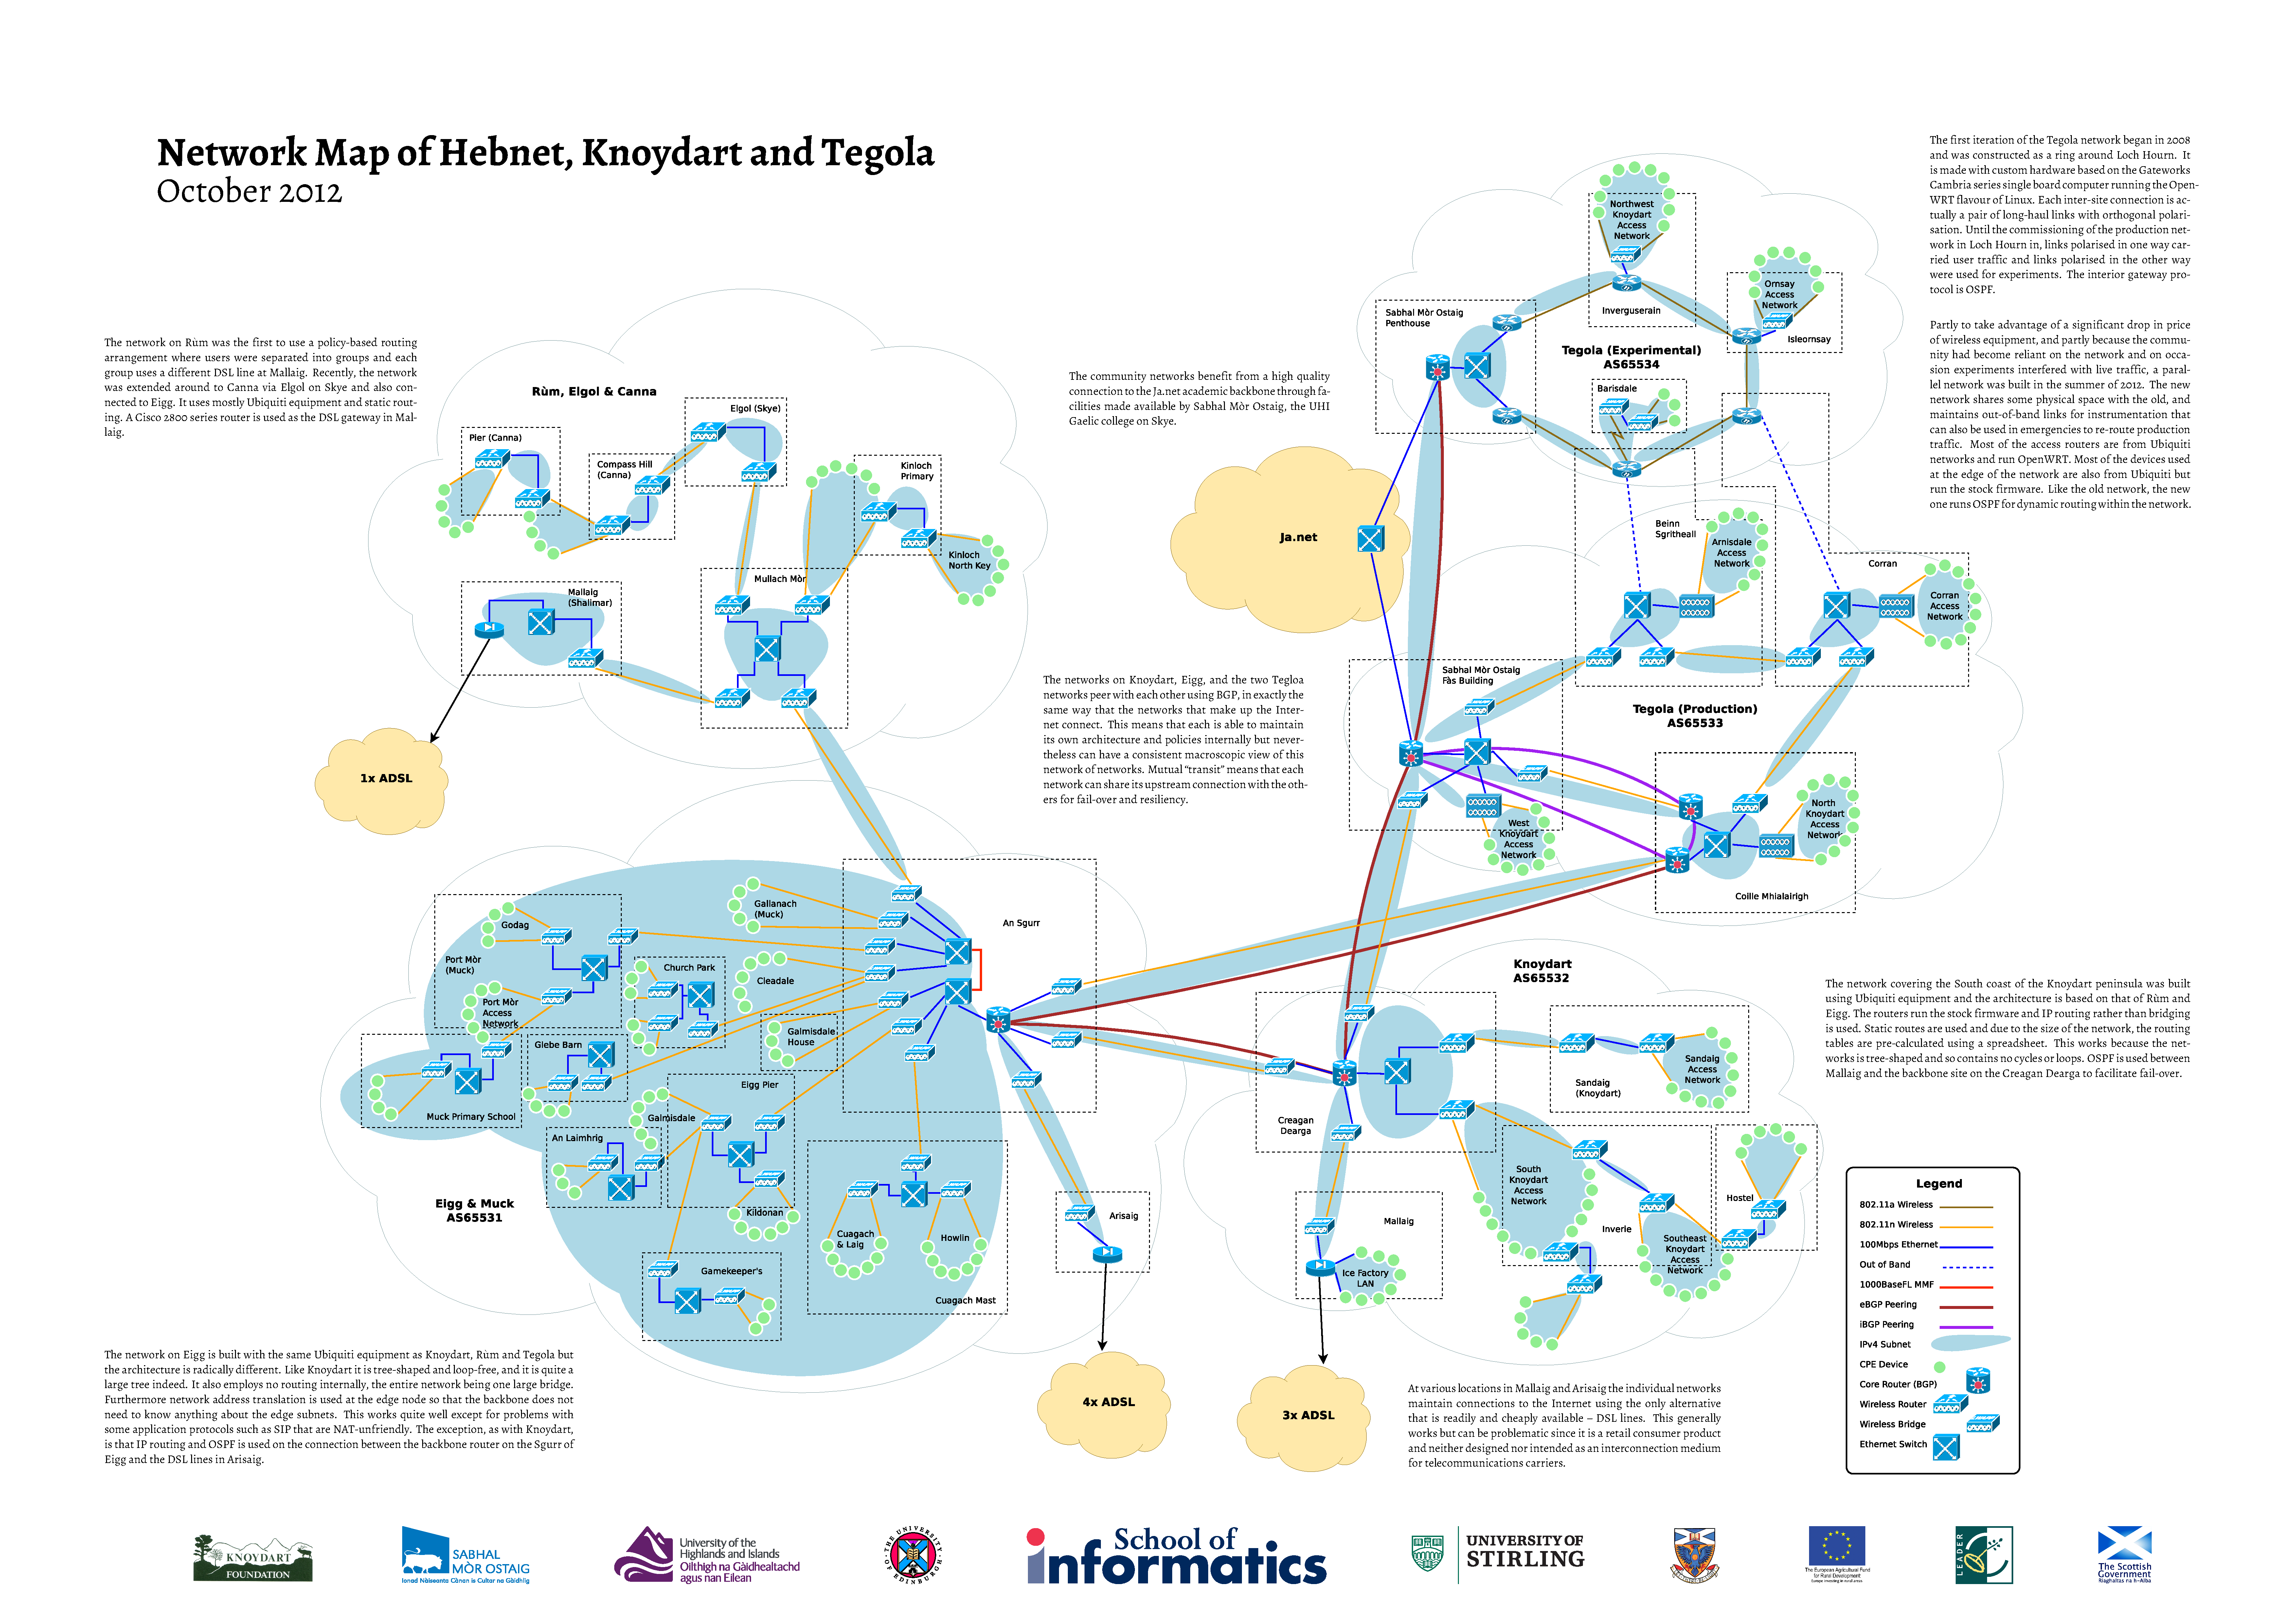
\includegraphics[height=\textwidth,angle=90]{big-map.pdf}
  \end{center}
  \caption{West Coast Confederation circa 2012}
  \label{fig:big_map}
\end{figure}

This structure can be repeated at different scales. Today, the
networks of Tegola, Knoydart and Hebnet all operate \textit{autonomous
  systems} and peer with each other and offer mutual transit. Being
connected in this way means that the internal details of how each of
them are built are not known about past their borders. This is
important because each is actually very different in construction and
operation. A now somewhat dated diagram that attempts to show this is
reproduced in figure \ref{fig:big_map}. Adding additional networks
means simply repeating this pattern of having a community encapsulated
in an autonomous system with links out to other communities and/or
backbone networks.

The current proposal is to take this confederation -- that is the
technical term for it -- and have it engage in peering and transit
relationships with the outside world on behalf of the confederation
members (i.e. the communities). This is exactly what \HUBS{} does
today in the South. The communities each have an autonomous system,
they connect amongst themselves and to the backbone, and all of this
is presented to the outside world, to the peering LAN at IX Scotland
and to our transit providers as a confederation. This is also exactly
the same structure as ja.net though they operate on a rather larger
scale.

So to do this, the confederation on the West Coast has to get to a
reasonable data centre where it is possible to have relationships with
as many other entities as possible. The first link will be from Fort
William to Edinburgh. The nature of this link is a long-distance
ethernet circuit, and there are several providers that can do this at
a reasonable price -- TalkTalk, Virgin and even BT. In the future,
when BT ethernet services are available at Kyle, a second circuit can
be established, ideally to a different datacentre. Manchester makes a
lot of sense for this because there are far more providers present
there than in Glasgow and it is relatively near to the Hibernia
trans-atlantic fibre as well as having good links to London and the
continent.

The proposal is that the West Coast confederation, yet to be
formalised into an organisation, and even named, will be an equal or
peer (in a wider sense than the narrow BGP protocol meaning) to
\HUBS{}. In the beginning, \HUBS{} will provide Internet transit to
the West Coast and this will mean that everybody benefits from the
economies of scale of increased traffic and it provides a quick way
for the West Coast confederation to take advantage of \HUBS{}'
existing relationships with other providers. In the longer term, when
the second circuit from Kyle is possible, the relationship will become
more symmetric with \HUBS{} being able to benefit from the West Coast
confederation's relationships in (say) Manchester.

Another, parallel evolutionary path has to do with the other project
in Argyll, where several communities are getting together and it seems
as though they might follow a similar model. It would be very easy to
connect to them directly with a wireless link from Eigg, and that will
establish a third route out from Oban. We have very little information
about those specific plans so this is somewhat speculative, but we are
hopeful that this can at least be discussed.

\subsection{Addressing}

IP addressing is crucially important for any Internet service. Indeed
with the current arrangement on the West Coast, where several networks
are sharing a small number of IP addresses -- in some cases just a
single one -- amongst their users, the case can be made that they are
not providing Internet access at all. There might be some hyperbole in
that statement, but not much.

Here are some reasons why IP addresses are important and using address
translation is not desireable:
\begin{itemize}
  \item Bad behaviour by one individual -- purposeful or accidental --
    and the reaction of others on the Internet affects everyone who is
    sharing the same address. Concretely, Google may stop answering
    search queries from the entire network because it thinks that it
    is one computer infected by a virus.
  \item Tracking usage to its source is very difficult. This is
    because of the information loss at the border where address
    translation happens. This means that it is not easily possible to
    notify the relevant user or take whatever action is necessary in
    case of complaints or legal action.
  \item While looking at web sites may work, other things that one
    might want to use the Internet for can break in a variety of
    ways. Particularly susceptible to this are VoIP (internet
    telephony) and GSM mobile pico-cells.
  \item Running services is not possible. Perhaps someone wants to run
    a web server to serve images from their camera looking at the
    beautiful scenery, or run an ssh server so that they can connect
    to their home computer while they are away elsewhere. Perhaps some
    parts of the network need to be instrumented and monitored, or
    data from a weather station or electricity generation system
    collected. These things are possible but very difficult without IP
    addresses.
  \item Having your own IP addresses means they are yours and do not
    belong to another entity or Internet Service Provider. When
    changing service providers you get to keep these addresses and
    don't have to re-number your network, a process that is rather
    painful. A minimum number of IP addresses is necessary to do this
    (a /24 block or 256 addresses).
\end{itemize}

Though IPv4 addresses are scarce and becoming difficult to obtain, it
is still possible for a new Internet Service Provider to obtain
them. This means joining the RIPE internet registry, and only one
new block of IPv4 addresses will be allocated -- a /22 network which
contains 1024 addresses. As a member of RIPE it is also possible to
purchase or lease additional addresses on the open market at a cost in
the neighbourhood of \pounds 10-20 at the time of writing.

Joining RIPE has a cost \cite{RIPECharges}. The sign-up fee is \euro
2000. Then there is an ongoing yearly membership fee of \euro 1750
plus \euro 50 per address block.

It is a requirement for obtaining IPv4 addresses to also implement
IPv6.
